% Toutes les valeurs viennent des sorties réelles de l'exécution du 28 octobre 2026 (resultats/sorties/).
% =====================================================================
\newpage
\section*{Introduction}
\phantomsection
\addcontentsline{toc}{section}{Introduction}

\noindent \textbf{MongoDB} est une base de données \textbf{NoSQL orientée documents}. Elle ne stocke pas de lignes dans des tables, mais des \textbf{documents} au format JSON (stockés en BSON), regroupés en \textbf{collections}, elles-mêmes rangées dans une \textbf{base}. Un document est un ensemble de paires champ~: valeur. Une valeur peut être un nombre, un texte, une date, un tableau ou un autre document~: les données se décrivent donc par imbrication, sans jointure. Deux documents d'une même collection n'ont pas obligatoirement les mêmes champs~: le schéma n'est pas imposé par la base.

\noindent Le tableau compare MongoDB au modèle relationnel et à Hive, vu dans le workshop précédent~:

\begin{tableau}{|>{\bfseries\raggedright\arraybackslash}p{\cw{0.18}}|>{\raggedright\arraybackslash}p{\cw{0.24}}|>{\raggedright\arraybackslash}p{\cw{0.28}}|>{\raggedright\arraybackslash}p{\cw{0.30}}|}
\rowcolor{tabentete}\normalfont \textbf{Notion} & \normalfont \textbf{Relationnel (SQL)} & \normalfont \textbf{Hive} & \normalfont \textbf{MongoDB} \\ \hline
Ensemble & Base & Base & Base \\ \hline
Regroupement & Table & Table (fichiers HDFS) & Collection \\ \hline
Unité de donnée & Ligne & Ligne d'un fichier & Document (JSON) \\ \hline
Schéma & Fixé avant l'écriture & Décrit dans le metastore, appliqué à la lecture & Libre, chaque document porte ses champs \\ \hline
Imbrication & Non, jointures & Types complexes limités & Documents et tableaux imbriqués \\ \hline
Langage & SQL & HiveQL & Méthodes JavaScript (\texttt{find}, \texttt{aggregate}) \\ \hline
\end{tableau}

\noindent La corbeille d'exercices comporte trois étapes~: installer MongoDB, importer trois jeux de données dans la base \texttt{corbeille}, puis répondre à seize questions avec le shell \textbf{mongosh}. Le compte-rendu commence par une étude des données, car leur forme décide des requêtes à écrire. Les valeurs données viennent de l'exécution réelle du 28~octobre 2026~; les réponses chiffrées (Q2 et Q4 à Q16) ont de plus été recalculées en Python, avec le même résultat.

% =====================================================================
\section*{Étude des données}
\phantomsection
\addcontentsline{toc}{section}{Étude des données}

\noindent Trois fichiers sont fournis. Chacun devient une collection de la base \texttt{corbeille}~:

\begin{tableau}{|>{\ttfamily\raggedright\arraybackslash}p{\cw{0.34}}|>{\raggedright\arraybackslash}p{\cw{0.09}}|>{\raggedleft\arraybackslash}p{\cw{0.14}}|>{\raggedright\arraybackslash}p{\cw{0.43}}|}
\rowcolor{tabentete}\normalfont \textbf{Fichier} & \normalfont \textbf{Format} & \normalfont \textbf{Documents} & \normalfont \textbf{Champs} \\ \hline
restaurants.json & JSON & 25\,357 & \texttt{name}, \texttt{restaurant\_id}, \texttt{borough}, \texttt{cuisine}, \texttt{address} (\texttt{building}, \texttt{coord}, \texttt{street}, \texttt{zipcode}), \texttt{grades} \\ \hline
netflix\_dataset.csv & CSV & 8\,807 & \texttt{show\_id}, \texttt{type}, \texttt{title}, \texttt{director}, \texttt{cast}, \texttt{country}, \texttt{date\_added}, \texttt{release\_year}, \texttt{rating}, \texttt{duration}, \texttt{listed\_in}, \texttt{description} \\ \hline
heightbycountry\_dataset.csv & CSV & 199 & \texttt{Rank}, \texttt{Country Name}, \texttt{Male Height in Cm}, \texttt{Female Height in Cm}, \texttt{Male Height in Ft}, \texttt{Female Height in Ft} \\ \hline
\end{tableau}

\noindent Le fichier \texttt{restaurants.json} contient un document par ligne. Ses documents sont imbriqués~: l'adresse est un sous-document, qui contient lui-même les coordonnées, et les notes forment un tableau de sous-documents. La figure montre cette structure, relevée sur le premier document de la collection.

\begin{center}
\begin{adjustbox}{max width=\linewidth}
\begin{tikzpicture}[every node/.style={font=\scriptsize}]
	\node[tbl=3.6cm] (r) {\tb{restaurants}{\pk{\_id}~: ObjectId \\ name~: texte \\ restaurant\_id~: texte \\ borough~: texte \\ cuisine~: texte \\ \textit{address}~: document \\ \textit{grades}~: tableau}};
	\node[sous=3.4cm, right=1.6cm of r, yshift=1.3cm] (a) {\tb{address}{building~: texte \\ street~: texte \\ zipcode~: texte \\ \textit{coord}~: document}};
	\node[sous=3.6cm, right=1.2cm of a] (c) {\tb{coord}{type~: \texttt{'Point'} \\ coordinates~: [longitude, latitude]}};
	\node[fait=3.4cm, below=0.6cm of a, xshift=0.0cm] (g) {\tb{grades (un élément par contrôle)}{date~: date \\ grade~: texte \\ score~: entier}};
	\draw[lien] (r.east) ++(0,0.6) -- (a.west);
	\draw[lien] (r.east) ++(0,-0.6) -- (g.west);
	\draw[lien] (a.east) -- (c.west);
\end{tikzpicture}
\end{adjustbox}\par\nobreak\smallskip
\small\textit{Figure~1 -- Structure d'un document de la collection \texttt{restaurants}~: \texttt{address} et \texttt{coord} sont imbriqués, \texttt{grades} est un tableau (4~éléments pour le premier document).}
\end{center}

\noindent Les données ont des particularités qui influencent les requêtes~:

\begin{tableau}{|>{\bfseries\raggedright\arraybackslash}p{\cw{0.20}}|>{\raggedright\arraybackslash}p{\cw{0.46}}|>{\raggedright\arraybackslash}p{\cw{0.34}}|}
\rowcolor{tabentete}\normalfont \textbf{Particularité} & \normalfont \textbf{Constat} & \normalfont \textbf{Conséquence} \\ \hline
\texttt{country} multi-valeurs & Un film a un ou plusieurs pays séparés par des virgules (par exemple « France, Belgium ») & Filtre par expression régulière en Q7 et Q8, découpage en Q12 \\ \hline
\texttt{duration} en texte & Valeur du type \texttt{'90 min'} ou \texttt{'2 Seasons'}, jamais un nombre & Comparaison avec la chaîne \texttt{'90 min'} \\ \hline
Champs vides & Les cases vides du CSV (\texttt{director}, \texttt{cast}, \texttt{country}\dots) sont importées comme des chaînes vides \texttt{''}, et non comme des champs absents & Les vides sont à exclure en Q12 \\ \hline
\texttt{borough} « Missing » & Valeur présente dans la collection, qui n'est pas un quartier & Q11~: 6 valeurs, dont 5 vrais quartiers \\ \hline
Cuisine \texttt{'American~'} & Une valeur avec une espace finale, distincte de \texttt{'American'} & Comptée telle quelle en Q9 \\ \hline
Cuisine mal encodée & \texttt{'Caf\~A\textcopyright/Coffee/Tea'} existe à côté de \texttt{'Café/Coffee/Tea'}, déjà dans le fichier source & Deux valeurs distinctes en Q9 \\ \hline
Noms de champs avec espaces & \texttt{Male Height in Cm}, \texttt{Country Name}\dots & Champ entre guillemets, \texttt{'\$Male Height in Cm'} en agrégation \\ \hline
\end{tableau}

% =====================================================================
\section*{Partie 1~: installation de MongoDB}
\phantomsection
\addcontentsline{toc}{section}{Partie 1~: installation de MongoDB}

\noindent L'énoncé demande la dernière version de MongoDB Community Server (alors la 5.0.6), la suite \textit{Database Tools}, puis l'ajout des dossiers \texttt{bin} au \texttt{PATH}. Voici ce qui a été installé et lancé sur le poste Windows~:

\begin{tableau}{|>{\bfseries\raggedright\arraybackslash}p{\cw{0.30}}|>{\raggedright\arraybackslash}p{\cw{0.30}}|>{\raggedright\arraybackslash}p{\cw{0.40}}|}
\rowcolor{tabentete}\normalfont \textbf{Élément} & \normalfont \textbf{Version utilisée} & \normalfont \textbf{Remarque} \\ \hline
Serveur MongoDB Community & 8.3 & Service Windows, écoute sur \texttt{localhost:27017} \\ \hline
\texttt{mongosh} & 2.14.0 & Shell des seize requêtes \\ \hline
MongoDB Database Tools & 100.20.0 & Archive zip, décompressée dans \texttt{C:\textbackslash Users\textbackslash mazou\textbackslash mongodb-tools} \\ \hline
\end{tableau}

\noindent Les écarts à l'énoncé sont les suivants~:
\begin{itemize}
	\item \textbf{Version}~: le serveur est en 8.3 et non en 5.0.6, puisque la 5.0.6 n'est plus la dernière version. Les requêtes de la corbeille n'utilisent que des fonctions anciennes (\texttt{find}, \texttt{distinct}, \texttt{aggregate}), mais elles n'ont pas été rejouées sur une 5.0.
	\item \textbf{Database Tools}~: installés depuis l'archive zip et non depuis un installateur. Le dossier n'est pas dans le \texttt{PATH}~: le script d'import appelle \texttt{mongoimport.exe} par son chemin complet.
\end{itemize}

% =====================================================================
\section*{Partie 2~: import des données}
\phantomsection
\addcontentsline{toc}{section}{Partie 2~: import des données}

\noindent L'import est écrit dans un script PowerShell, \texttt{import.ps1}, qui peut être rejoué grâce à l'option \texttt{-{}-drop} (elle supprime la collection avant de la recréer). Les deux fichiers CSV utilisent \texttt{-{}-type csv -{}-headerline}, qui prend la première ligne comme noms de champs. Le fichier JSON, qui contient un document par ligne, s'importe sans option de format~:

\begin{minted}{powershell}
mongoimport --uri mongodb://localhost:27017 --db corbeille --collection netflix --drop --type csv --headerline --file netflix_dataset.csv
mongoimport --uri mongodb://localhost:27017 --db corbeille --collection height --drop --type csv --headerline --file heightbycountry_dataset.csv
mongoimport --uri mongodb://localhost:27017 --db corbeille --collection restaurants --drop --file restaurants.json
\end{minted}

\noindent L'énoncé ne cite que \texttt{netflix} et \texttt{restaurants}, mais les questions 13 à 16 portent sur les tailles~: la collection \texttt{height} est donc importée aussi. Le résultat réel est le suivant, sans aucun échec~:

\begin{tableau}{|>{\ttfamily\raggedright\arraybackslash}p{\cw{0.30}}|>{\raggedleft\arraybackslash}p{\cw{0.30}}|>{\raggedleft\arraybackslash}p{\cw{0.40}}|}
\rowcolor{tabentete}\normalfont \textbf{Collection} & \normalfont \textbf{Documents importés} & \normalfont \textbf{Documents en échec} \\ \hline
netflix & 8\,807 & 0 \\ \hline
height & 199 & 0 \\ \hline
restaurants & 25\,357 & 0 \\ \hline
\end{tableau}

\noindent Ces nombres sont ceux annoncés par l'énoncé (25\,357, 8\,807 et 199). Avec un fichier CSV, \texttt{mongoimport} devine le type de chaque valeur. La capture montre l'exécution réelle de \texttt{import.ps1} dans une console PowerShell~; elle a été refaite le 28~octobre 2026 à 16\,h~55 et donne les mêmes nombres. Deux contrôles confirment que le résultat est correct~: \texttt{release\_year} est un entier pour les 8\,807 documents (requête de vérification sur \texttt{\$type}), et les tailles sont numériques, puisque leur moyenne se calcule (Q13).

\begin{center}
\adjustbox{max width=\linewidth, max height=0.3\textheight}{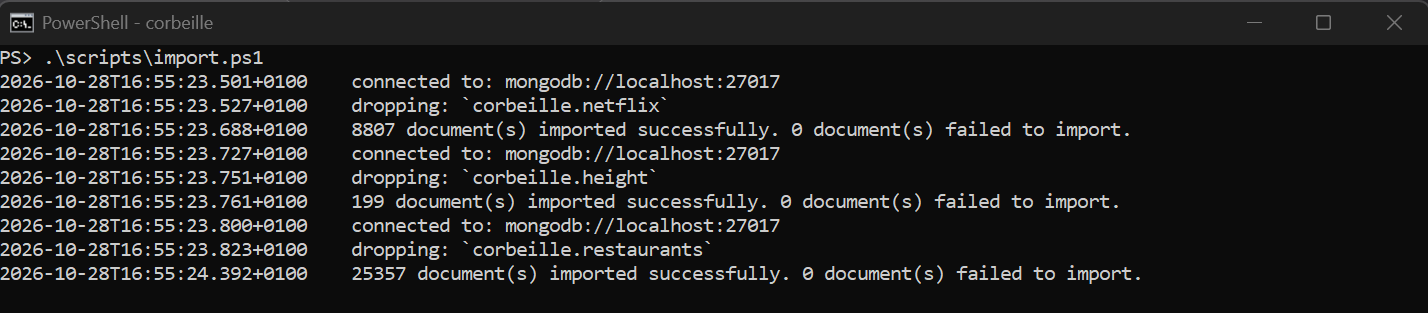
\includegraphics{contents/img/captures/mongoimport.png}}\par\nobreak\smallskip
\small\textit{Figure~2 -- Exécution de \texttt{import.ps1} (console PowerShell)~: trois collections importées, 0~échec.}
\end{center}

% =====================================================================
\section*{Partie 3~: requêtes}
\phantomsection
\addcontentsline{toc}{section}{Partie 3~: requêtes}

\noindent Les seize requêtes sont écrites dans \texttt{requetes.js}, lancé par \texttt{mongosh corbeille -{}-quiet -{}-file requetes.js}. Pour les types \og films \fg{} et \og séries TV \fg{}, la collection \texttt{netflix} utilise le champ \texttt{type}, qui vaut \texttt{'Movie'} ou \texttt{'TV Show'}.

\subsection*{1. Découverte de la base (Q1 à Q3)}
\phantomsection
\addcontentsline{toc}{subsection}{1. Découverte de la base (Q1 à Q3)}

\noindent \textbf{Q1. Liste des collections de la base.}

\begin{minted}{javascript}
db.getCollectionNames()
\end{minted}

\noindent Résultat~: \texttt{['restaurants', 'netflix', 'height']}. La base contient bien les trois collections importées (l'ordre de la liste n'est pas garanti~: après le rejeu de l'import de la capture, les collections sont renvoyées dans l'ordre \texttt{restaurants}, \texttt{height}, \texttt{netflix}).

\medskip
\needspace{8\baselineskip}
\noindent \textbf{Q2. Nombre de documents des collections \texttt{netflix} et \texttt{restaurants}.}

\begin{minted}{javascript}
db.netflix.countDocuments({})
db.restaurants.countDocuments({})
\end{minted}

\noindent Résultat~: \textbf{8\,807} documents dans \texttt{netflix} et \textbf{25\,357} dans \texttt{restaurants}, soit les nombres de l'énoncé. La capture montre ces deux premières requêtes dans mongosh, avec la liste des collections.

\begin{center}
\adjustbox{max width=\linewidth, max height=0.3\textheight}{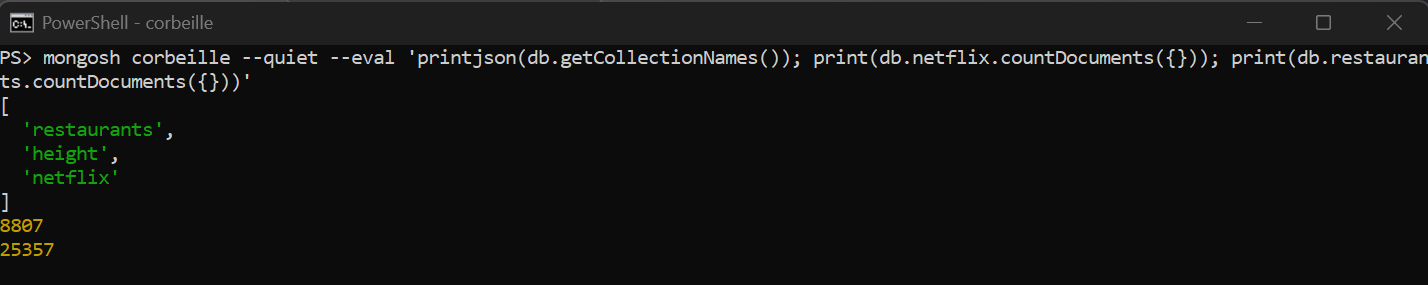
\includegraphics{contents/img/captures/q01_q02.png}}\par\nobreak\smallskip
\small\textit{Figure~3 -- Q1 et Q2 dans la console~: liste des collections, puis \texttt{countDocuments} sur \texttt{netflix} et \texttt{restaurants}.}
\end{center}

\medskip
\needspace{8\baselineskip}
\noindent \textbf{Q3. Un document de chaque collection et la liste de leurs champs.}

\begin{minted}{javascript}
const docNetflix = db.netflix.findOne();
print("Champs netflix : " + Object.keys(docNetflix).join(", "));
const docResto = db.restaurants.findOne();
print("Champs restaurants : " + Object.keys(docResto).join(", "));
\end{minted}

\noindent Les champs relevés sont les suivants. Le champ \texttt{\_id} est ajouté par MongoDB à chaque document~:

\begin{tableau}{|>{\bfseries\raggedright\arraybackslash}p{\cw{0.17}}|>{\ttfamily\raggedright\arraybackslash}p{\cw{0.83}}|}
\rowcolor{tabentete}\normalfont \textbf{Collection} & \normalfont \textbf{Champs du document} \\ \hline
netflix & \_id, show\_id, type, title, director, cast, country, date\_added, release\_year, rating, duration, listed\_in, description \\ \hline
restaurants & \_id, address, borough, cuisine, grades, name, restaurant\_id \\ \hline
\end{tableau}

\noindent Le document \texttt{netflix} obtenu est la série \texttt{s2} (champ \texttt{cast} abrégé)~:

\begin{tableau}{|>{\ttfamily\raggedright\arraybackslash}p{\cw{0.20}}|>{\raggedright\arraybackslash}p{\cw{0.80}}|}
\rowcolor{tabentete}\normalfont \textbf{Champ} & \normalfont \textbf{Valeur} \\ \hline
show\_id & s2 \\ \hline
type & TV Show \\ \hline
title & Blood \& Water \\ \hline
director & (chaîne vide) \\ \hline
cast & Ama Qamata, Khosi Ngema, Gail Mabalane, \dots (19~noms) \\ \hline
country & South Africa \\ \hline
date\_added & September 24, 2021 \\ \hline
release\_year & 2021 \\ \hline
rating, duration & TV-MA, 2 Seasons \\ \hline
\end{tableau}

\noindent Le document \texttt{restaurants} obtenu est \og Riviera Caterer \fg{}, à Brooklyn, avec la cuisine \texttt{'American~'} et quatre notes (de 2011 à 2014). Sa structure est celle de la figure~1. On note que \texttt{director} est présent mais vide~: c'est la conséquence de l'import CSV décrite plus haut.

\subsection*{2. Collection netflix (Q4 à Q8 et Q12)}
\phantomsection
\addcontentsline{toc}{subsection}{2. Collection netflix (Q4 à Q8 et Q12)}

\noindent \textbf{Q4. Nombre de films sortis en 2016.}

\begin{minted}{javascript}
db.netflix.countDocuments({ type: "Movie", release_year: 2016 })
db.netflix.countDocuments({ release_year: 2016 })   // variante
\end{minted}

\noindent Résultat~: \textbf{658 films}. La question parle de films~; la variante qui ne filtre pas sur le type compte aussi les séries et donne 902 documents sortis en 2016.

\medskip
\needspace{8\baselineskip}
\noindent \textbf{Q5 et Q6. Nombre de films et de séries TV.}

\begin{minted}{javascript}
db.netflix.countDocuments({ type: "Movie" })
db.netflix.countDocuments({ type: "TV Show" })
\end{minted}

\noindent Résultat~: \textbf{6\,131 films} et \textbf{2\,676 séries TV}. Leur somme, 8\,807, est le nombre total de documents~: il n'y a pas d'autre type. Les films représentent environ 70\,\% du catalogue (6\,131 sur 8\,807).

\medskip
\needspace{8\baselineskip}
\noindent \textbf{Q7. Nombre de films français dont la durée est de 90 minutes.} Le champ \texttt{country} peut contenir plusieurs pays~: le filtre cherche donc \og France \fg{} dans le texte avec une expression régulière. Comme \texttt{duration} est un texte, on compare avec \texttt{'90 min'}.

\begin{minted}{javascript}
db.netflix.countDocuments({ type: "Movie", country: /France/, duration: "90 min" })
db.netflix.countDocuments({ type: "Movie", country: "France", duration: "90 min" })   // variante
\end{minted}

\noindent Résultat~: \textbf{6 films}. La variante, qui exige que \texttt{country} soit exactement \texttt{'France'}, donne \textbf{0}~: les films français de 90 minutes ont tous plusieurs pays de production. Un filtre sur la valeur exacte aurait donc donné une réponse fausse sans avertissement.

\medskip
\needspace{8\baselineskip}
\noindent \textbf{Q8. Nombre de films américains sortis depuis 2020.} Même principe pour le pays, avec \texttt{\$gte} sur l'année.

\begin{minted}{javascript}
db.netflix.countDocuments({ type: "Movie", country: /United States/, release_year: { $gte: 2020 } })
\end{minted}

\noindent Résultat~: \textbf{265 films}. \og Depuis 2020 \fg{} est interprété comme 2020 inclus (\texttt{\$gte}).

\medskip
\needspace{14\baselineskip}
\noindent \textbf{Q12. Nombre de pays pour lesquels la collection contient au moins un film.} La question est la plus délicate~: un champ \texttt{country} contient une liste de pays. Il faut donc découper le texte, mettre un pays par document, nettoyer, puis compter les valeurs distinctes. La figure montre les étapes du pipeline d'agrégation.

\begin{center}
\begin{adjustbox}{max width=\linewidth}
\begin{tikzpicture}[node distance=0.55cm, every node/.style={font=\scriptsize}]
	\node[cmp=2.0cm] (m) {\textbf{\$match}\\ films, \texttt{country} texte};
	\node[cmp=2.0cm, right=of m] (s) {\textbf{\$project}\\ \texttt{\$split} sur \texttt{','}};
	\node[cmp=2.0cm, right=of s] (u) {\textbf{\$unwind}\\ un pays par document};
	\node[cmp=2.0cm, right=of u] (t) {\textbf{\$project}\\ \texttt{\$trim} des espaces};
	\node[cmp=2.0cm, right=of t] (g) {\textbf{\$match}, \textbf{\$group}\\ vides exclus, \texttt{\_id} = pays};
	\node[cmp=1.6cm, right=of g, fill=title2!12, draw=title1] (c) {\textbf{\$count}\\ \texttt{n}};
	\draw[flux] (m) -- (s);
	\draw[flux] (s) -- (u);
	\draw[flux] (u) -- (t);
	\draw[flux] (t) -- (g);
	\draw[flux] (g) -- (c);
\end{tikzpicture}
\end{adjustbox}\par\nobreak\smallskip
\small\textit{Figure~5 -- Pipeline d'agrégation de Q12~: de la liste de pays d'un film au nombre de pays distincts.}
\end{center}

\begin{minted}{javascript}
db.netflix.aggregate([
  { $match: { type: "Movie" } },
  { $match: { country: { $type: "string" } } },
  { $project: { pays: { $split: ["$country", ","] } } },
  { $unwind: "$pays" },
  { $project: { pays: { $trim: { input: "$pays" } } } },
  { $match: { pays: { $ne: "" } } },
  { $group: { _id: "$pays" } },
  { $count: "n" }
])
\end{minted}

\noindent Le \texttt{\$trim} est nécessaire~: après un découpage sur la virgule, \texttt{' Belgium'} (avec une espace) et \texttt{'Belgium'} seraient comptés comme deux pays. Le second \texttt{\$match} retire les pays vides, issus des champs \texttt{country} vides. Résultat~: \textbf{117 pays} avec au moins un film. La variante sans filtre sur le type (films et séries) donne 122 pays. La capture montre le fichier d'agrégation et son résultat (dans le fichier, l'agrégation est enveloppée dans \texttt{printjson(...toArray())} pour afficher le résultat).

\begin{center}
\adjustbox{max width=\linewidth, max height=0.3\textheight}{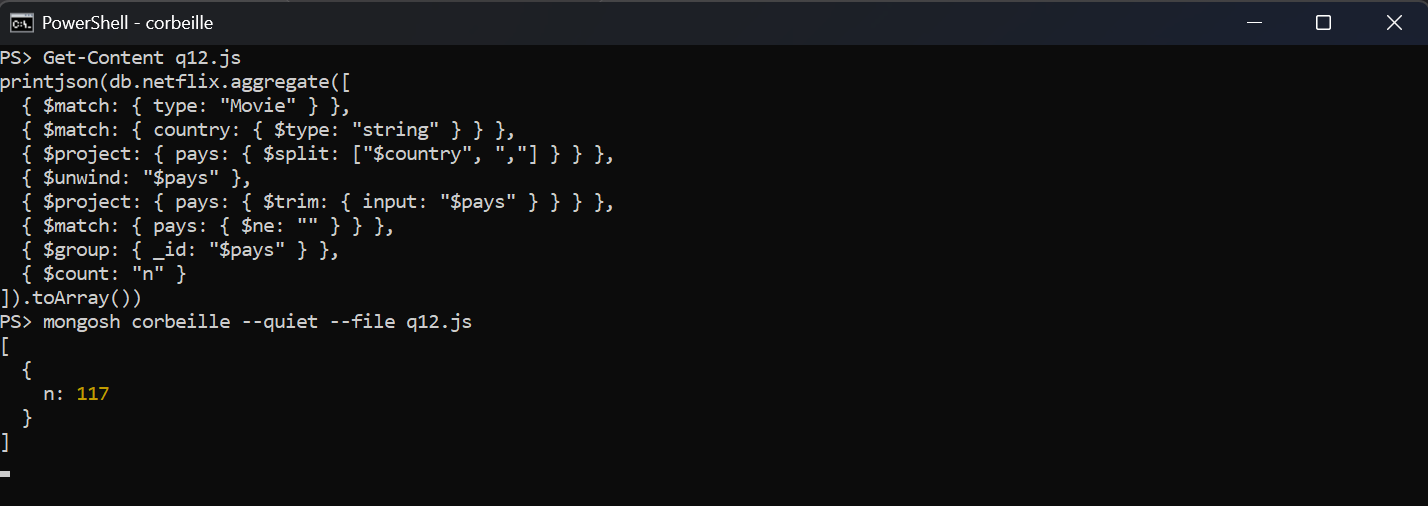
\includegraphics{contents/img/captures/q12.png}}\par\nobreak\smallskip
\small\textit{Figure~6 -- Q12 dans mongosh~: pipeline d'agrégation et résultat \texttt{n: 117}.}
\end{center}

\subsection*{3. Collection restaurants (Q9 à Q11)}
\phantomsection
\addcontentsline{toc}{subsection}{3. Collection restaurants (Q9 à Q11)}

\noindent \textbf{Q9. Liste des types de restaurants (cuisine).} La méthode \texttt{distinct} renvoie les valeurs différentes d'un champ, triées.

\begin{minted}{javascript}
const cuisines = db.restaurants.distinct("cuisine");
print("Nombre de cuisines distinctes : " + cuisines.length);
\end{minted}

\noindent Résultat~: \textbf{85 valeurs distinctes}. La liste complète est trop longue pour être reproduite~; le tableau donne ses extrémités et les cas particuliers.

\begin{tableau}{|>{\bfseries\raggedright\arraybackslash}p{\cw{0.22}}|>{\raggedright\arraybackslash}p{\cw{0.78}}|}
\rowcolor{tabentete}\normalfont \textbf{Partie de la liste} & \normalfont \textbf{Valeurs} \\ \hline
Début & Afghan, African, \texttt{'American~'}, Armenian, Asian, Australian, Bagels/Pretzels, Bakery \\ \hline
Cas particuliers & \texttt{'American~'} (espace finale), \texttt{'Caf\~A\textcopyright/Coffee/Tea'} et \texttt{'Café/Coffee/Tea'} \\ \hline
Valeurs composées & Chinese/Cuban, Chinese/Japanese, Creole/Cajun, Pizza/Italian, Hotdogs/Pretzels \\ \hline
Valeurs génériques & Not Listed/Not Applicable, Other \\ \hline
Fin & Thai, Turkish, Vegetarian, Vietnamese/Cambodian/Malaysia \\ \hline
\end{tableau}

\noindent Les 85 valeurs sont des valeurs brutes. Si les deux variantes de \og Café \fg{} étaient regroupées, la liste compterait 84 types. Ces défauts sont signalés mais non corrigés~: la question demande la liste telle qu'elle est stockée.

\medskip
\needspace{8\baselineskip}
\noindent \textbf{Q10. Nombre de restaurants dans le Queens.}

\begin{minted}{javascript}
db.restaurants.countDocuments({ borough: "Queens" })
\end{minted}

\noindent Résultat~: \textbf{5\,656 restaurants}, soit environ 22\,\% des 25\,357 restaurants de la collection. La capture montre l'exécution de Q7 (résultat 6) et de Q10 depuis un fichier, lancé avec \texttt{mongosh -{}-file}.

\begin{center}
\adjustbox{max width=\linewidth, max height=0.3\textheight}{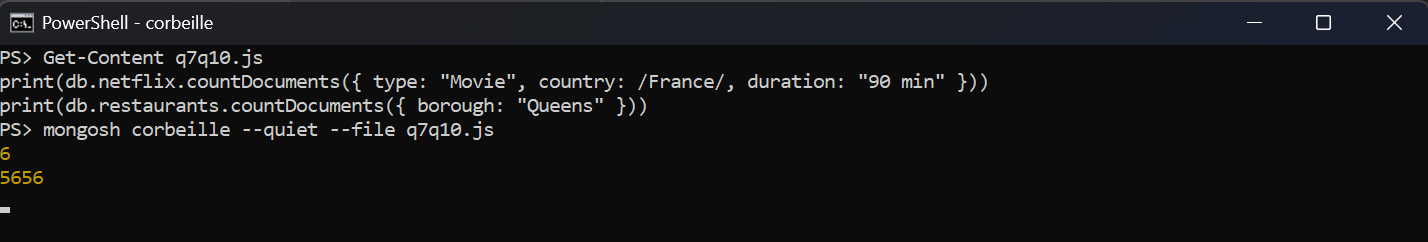
\includegraphics{contents/img/captures/q07_q10.png}}\par\nobreak\smallskip
\small\textit{Figure~4 -- Q7 (6~films français de 90~min) et Q10 (5\,656 restaurants dans le Queens), exécutés dans mongosh.}
\end{center}

\medskip
\needspace{8\baselineskip}
\noindent \textbf{Q11. Liste des quartiers qui contiennent au moins un restaurant.}

\begin{minted}{javascript}
db.restaurants.distinct("borough")
\end{minted}

\noindent Résultat~: \textbf{6 valeurs}, \texttt{'Bronx'}, \texttt{'Brooklyn'}, \texttt{'Manhattan'}, \texttt{'Missing'}, \texttt{'Queens'} et \texttt{'Staten Island'}. \texttt{'Missing'} n'est pas un quartier~: c'est la valeur des restaurants dont le quartier est inconnu. New York compte cinq quartiers, ce qui correspond aux cinq autres valeurs.

\subsection*{4. Collection height (Q13 à Q16)}
\phantomsection
\addcontentsline{toc}{subsection}{4. Collection height (Q13 à Q16)}

\noindent \textbf{Q13 et Q14. Taille moyenne des hommes et des femmes, tous pays confondus.} L'opérateur \texttt{\$avg} calcule la moyenne dans un \texttt{\$group} sans clé (\texttt{\_id: null}). Les noms de champs contiennent des espaces~: ils sont écrits entre guillemets, précédés de \texttt{\$}.

\begin{minted}{javascript}
db.height.aggregate([{ $group: { _id: null, m: { $avg: "$Male Height in Cm" } } }])
db.height.aggregate([{ $group: { _id: null, m: { $avg: "$Female Height in Cm" } } }])
\end{minted}

\noindent Résultat~: \textbf{173,09~cm} pour les hommes (valeur brute 173,08904522613065) et \textbf{160,94~cm} pour les femmes (160,9429145728643). Il s'agit d'une moyenne simple des 199 pays, non pondérée par la population~: ce n'est pas la taille moyenne des habitants du monde. Les hommes sont en moyenne plus grands de 12,15~cm.

\medskip
\needspace{14\baselineskip}
\noindent \textbf{Q15 et Q16. Pays aux hommes les plus petits et aux femmes les plus grandes.} Un tri suivi de \texttt{limit(3)} donne le premier pays et les deux suivants, pour vérifier l'absence d'ex æquo.

\begin{minted}{javascript}
db.height.find({}, { _id: 0, "Country Name": 1, "Male Height in Cm": 1 })
  .sort({ "Male Height in Cm": 1 }).limit(3)
db.height.find({}, { _id: 0, "Country Name": 1, "Female Height in Cm": 1 })
  .sort({ "Female Height in Cm": -1 }).limit(3)
\end{minted}

\begin{tableau}{|>{\bfseries\centering\arraybackslash}p{\cw{0.08}}|>{\raggedright\arraybackslash}p{\cw{0.25}}|>{\raggedleft\arraybackslash}p{\cw{0.20}}|>{\bfseries\centering\arraybackslash}p{\cw{0.08}}|>{\raggedright\arraybackslash}p{\cw{0.25}}|>{\raggedleft\arraybackslash}p{\cw{0.14}}|}
\rowcolor{tabentete}\normalfont \textbf{Rang} & \normalfont \textbf{Hommes, plus petits} & \normalfont \textbf{Taille (cm)} & \normalfont \textbf{Rang} & \normalfont \textbf{Femmes, plus grandes} & \normalfont \textbf{Taille (cm)} \\ \hline
1 & Timor-Leste & 160,13 & 1 & Netherlands & 170,36 \\ \hline
2 & Laos & 162,78 & 2 & Montenegro & 169,96 \\ \hline
3 & Solomon Islands & 163,07 & 3 & Denmark & 169,47 \\ \hline
\end{tableau}

\noindent Les réponses sont \textbf{Timor-Leste, 160,13~cm} (Q15) et \textbf{Netherlands, 170,36~cm} (Q16). Il n'y a pas d'ex æquo~: les tailles du deuxième pays sont différentes. Les Pays-Bas sont aussi au rang~1 du fichier source pour les hommes (183,78~cm). La capture montre l'exécution de Q15 et Q16 (script de sortie compact, trois pays par tri), puis la dernière figure résume les résultats de Q5, Q6 et de Q13 à Q16.

\begin{center}
\adjustbox{max width=\linewidth, max height=0.3\textheight}{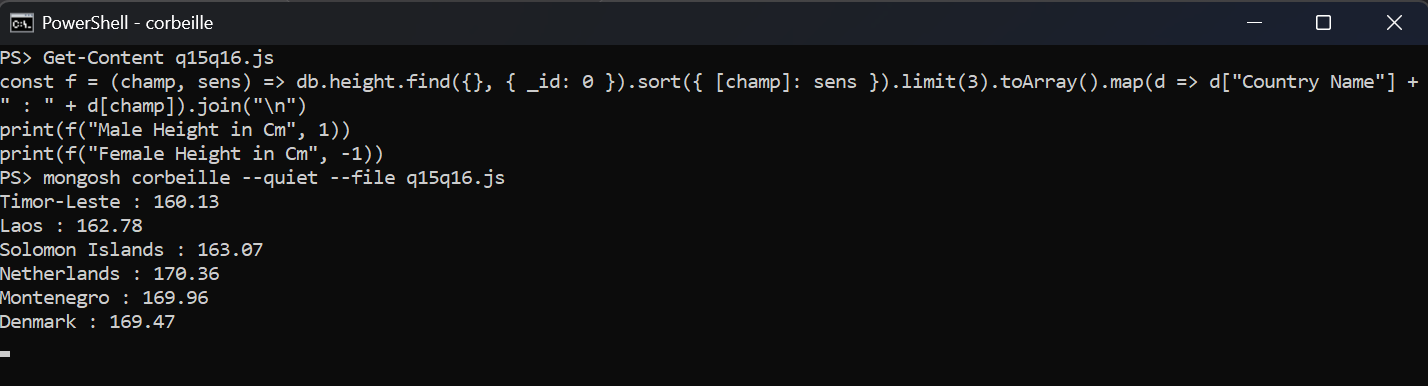
\includegraphics{contents/img/captures/q15_q16.png}}\par\nobreak\smallskip
\small\textit{Figure~7 -- Q15 et Q16 dans mongosh~: les trois pays aux hommes les plus petits, puis aux femmes les plus grandes.}
\end{center}


\begin{center}
\begin{minipage}{0.40\textwidth}
\centering
\begin{tikzpicture}
\begin{axis}[ybar, width=\linewidth, height=5.6cm, symbolic x coords={Films,Séries}, xtick=data, ymin=0, ymax=7500, enlarge x limits=0.5, bar width=0.8cm,
	ylabel={Nombre de titres}, ylabel style={font=\scriptsize}, tick label style={font=\scriptsize}, scaled y ticks=false, yticklabel style={/pgf/number format/fixed, /pgf/number format/1000 sep=\,},
	nodes near coords, nodes near coords style={font=\tiny}, every node near coord/.append style={/pgf/number format/fixed, /pgf/number format/1000 sep=\,}]
\addplot[fill=title1!70] coordinates {(Films,6131) (Séries,2676)};
\end{axis}
\end{tikzpicture}
\end{minipage}\hfill
\begin{minipage}{0.56\textwidth}
\centering
\begin{tikzpicture}
\begin{axis}[ybar, width=\linewidth, height=5.6cm, symbolic x coords={Moyenne,Extrême}, xtick=data, ymin=150, ymax=185, enlarge x limits=0.5, bar width=0.6cm,
	ylabel={Taille (cm)}, ylabel style={font=\scriptsize}, tick label style={font=\scriptsize}, legend style={font=\tiny, at={(0.5,1.03)}, anchor=south, legend columns=2},
	nodes near coords, nodes near coords style={font=\tiny}, every node near coord/.append style={/pgf/number format/fixed, /pgf/number format/precision=2}]
\addplot[fill=title1!70] coordinates {(Moyenne,173.09) (Extrême,160.13)};
\addplot[fill=orange!70] coordinates {(Moyenne,160.94) (Extrême,170.36)};
\legend{Hommes, Femmes}
\end{axis}
\end{tikzpicture}
\end{minipage}\par\nobreak\smallskip
\small\textit{Figure~8 -- À gauche~: films et séries de la collection \texttt{netflix} (Q5, Q6). À droite~: tailles en cm, moyenne des 199 pays (Q13, Q14) et valeur extrême (Q15~: hommes les plus petits, Timor-Leste~; Q16~: femmes les plus grandes, Netherlands). L'axe commence à 150~cm.}
\end{center}

% =====================================================================
\section*{Synthèse et écarts à l'énoncé}
\phantomsection
\addcontentsline{toc}{section}{Synthèse et écarts à l'énoncé}

\subsection*{1. Réponses}
\phantomsection
\addcontentsline{toc}{subsection}{1. Réponses}

\noindent Le tableau regroupe les réponses aux seize questions, telles que renvoyées par \texttt{mongosh}~:

\begin{tableau}{|>{\bfseries\centering\arraybackslash}p{\cw{0.07}}|>{\raggedright\arraybackslash}p{\cw{0.55}}|>{\raggedleft\arraybackslash}p{\cw{0.38}}|}
\rowcolor{tabentete}\normalfont \textbf{Q} & \normalfont \textbf{Question} & \normalfont \textbf{Réponse} \\ \hline
1 & Collections de la base & restaurants, netflix, height \\ \hline
2 & Documents de netflix et de restaurants & 8\,807 et 25\,357 \\ \hline
3 & Champs d'un document & 13 champs (netflix), 7 (restaurants) \\ \hline
4 & Films sortis en 2016 & 658 \\ \hline
5 & Films & 6\,131 \\ \hline
6 & Séries TV & 2\,676 \\ \hline
7 & Films français de 90 min & 6 \\ \hline
8 & Films américains depuis 2020 & 265 \\ \hline
9 & Types de cuisine & 85 valeurs distinctes \\ \hline
10 & Restaurants dans le Queens & 5\,656 \\ \hline
11 & Quartiers & 6 valeurs (dont \og Missing \fg) \\ \hline
12 & Pays avec au moins un film & 117 \\ \hline
13 & Taille moyenne des hommes & 173,09 cm \\ \hline
14 & Taille moyenne des femmes & 160,94 cm \\ \hline
15 & Hommes les plus petits & Timor-Leste, 160,13 cm \\ \hline
16 & Femmes les plus grandes & Netherlands, 170,36 cm \\ \hline
\end{tableau}

\subsection*{2. Écarts et choix d'interprétation}
\phantomsection
\addcontentsline{toc}{subsection}{2. Écarts et choix d'interprétation}

\begin{itemize}[midpenalty=0, endpenalty=0]
	\item \textbf{Version et installation}~: serveur 8.3, \texttt{mongosh} 2.14.0 et Database Tools 100.20.0 (archive zip, chemin complet de \texttt{mongoimport}, \texttt{PATH} inchangé), au lieu de la 5.0.6 de l'énoncé.
	\item \textbf{Collection \texttt{height}}~: importée en plus de \texttt{netflix} et \texttt{restaurants}, car Q13 à Q16 en ont besoin.
	\item \textbf{\og Films \fg{} et \og séries \fg{}}~: interprétés comme \texttt{type = 'Movie'} et \texttt{type = 'TV Show'}. Les variantes sans filtre de type sont données pour Q4 (902) et Q12 (122).
	\item \textbf{Q7 et Q8}~: pays multiples, d'où un filtre par expression régulière (le filtre exact donne 0 en Q7)~; \og depuis 2020 \fg{} est lu comme 2020 inclus.
	\item \textbf{Q9, Q11, Q13 et Q14}~: valeurs brutes sans nettoyage (espace finale, variante mal encodée, \og Missing \fg), moyenne simple sur les 199 pays arrondie à deux décimales.
	\item \textbf{Q3}~: \texttt{findOne()} a renvoyé la série \texttt{s2} et non \texttt{s1}, car l'ordre naturel n'est pas garanti~; seule la liste des champs est la réponse.
\end{itemize}

% =====================================================================
\section*{Conclusion}
\phantomsection
\addcontentsline{toc}{section}{Conclusion}

\noindent Cette corbeille a permis de manipuler MongoDB en ligne de commande, de l'installation aux seize requêtes~:
\begin{enumerate}
	\item \textbf{l'import}~: \texttt{mongoimport} charge un CSV ou un JSON dans une collection en une commande, sans schéma préalable. Les 34\,363 documents sont arrivés sans échec~;
	\item \textbf{les requêtes simples}~: \texttt{countDocuments}, \texttt{distinct} et \texttt{find} avec filtre, tri et limite répondent à la plupart des questions~;
	\item \textbf{l'agrégation}~: \texttt{\$group}, \texttt{\$split}, \texttt{\$unwind} et \texttt{\$trim} sont nécessaires dès que la donnée n'est pas dans la forme attendue, comme les pays multiples de Q12.
\end{enumerate}

\noindent Le point à retenir est que l'absence de schéma impose de bien connaître les données avant de les interroger~: un champ multi-valeurs, une durée en texte, des cases vides importées comme des chaînes ou une valeur \og Missing \fg{} donnent des réponses fausses si l'on ne les anticipe pas. Par rapport à Hive, MongoDB se prête mieux aux documents imbriqués comme les restaurants et se charge plus simplement~; Hive reste plus proche du SQL pour des jointures et des agrégats sur des tables régulières.
